\documentclass[11pt,a4paper]{article}
\usepackage[T1]{fontenc}
\usepackage[margin=2.3cm]{geometry}
\usepackage{amsmath,amssymb}
\usepackage{graphicx}
\usepackage[dvipsnames]{xcolor}
\usepackage{enumitem}
\usepackage[colorlinks=true,linkcolor=blue,urlcolor=blue]{hyperref}
\setlength{\parskip}{0.6em}
\setlength{\parindent}{0pt}
\begin{document}

\begin{center}{\LARGE\bfseries opencalculus}\\[0.4em]{\large See derivatives and integrals as slopes and areas on a moving car's graph.}\\[0.2em]\small PAN IIT OSS explainer \textbullet{} secondary school to diploma / undergraduate (levels 3-5)\end{center}

\section*{Why this exists}
Calculus is the mathematics of change and accumulation. This explainer follows a moving car: the slope of its distance graph is its speed and the area under its speed graph is the distance it covers, then shows how computers estimate both and how large their errors are.

\section*{The end goal}
See derivatives and integrals as slopes and areas on a moving car's graph. The end goal is to see derivatives and integrals as slopes and areas on a moving car's graph. The same ideas drive physics (velocity, work, charge), engineering (signals, control) and data science (rates and totals from measurements).

\section*{How the three sessions build up}
\begin{enumerate}[nosep]
\item \textbf{Session 1: Slope is speed, area is distance} (Level 1, conceptual interactive model, 60 min).
\item \textbf{Session 2: Derivative and integral as limits} (Level 2, mathematical engineering model, 75 min).
\item \textbf{Session 3: Numerical slopes and areas, and their errors} (Level 3, simulation and validation, 90 min).
\end{enumerate}

\section{Session 1: Slope is speed, area is distance}

\subsection*{A. Real-world problem}
A car's speedometer tells you how fast you go but not how far you have come; its odometer tells you how far but not how fast. If you only had a record of one of them, could you rebuild the other? That question is the whole of calculus in disguise: going from distance to speed is differentiation, going from speed to distance is integration. In this session you do both with nothing but slopes and areas.

\subsection*{B. Concept and theory}
Speed is distance divided by time. On a distance-time graph, 'distance divided by time' is rise over run, the slope. When the speed changes, the slope changes from moment to moment: the speed at a moment is the slope of the tangent line touching the curve there. Going the other way, distance equals speed times time. On a speed-time graph that is width times height, the area of a rectangle; if the speed changes we cut the time into slices and add up the areas (a trapezoid for a straight-line change). The unit of the area is s * m/s = m. Our car starts at rest and its speed is known at 0, 2, 4 and 6 s, with straight lines in between.

\begin{itemize}[nosep]
\item t: time since the start (s)
\item v(t): speed of the car at time t (m/s)
\item x(t): distance travelled since the start, up to time t (m)
\item slope: rise over run of the distance graph (m/s)
\item area: area under the speed graph (m)
\end{itemize}

\begin{equation*}
v=\frac{\Delta x}{\Delta t}\quad\text{(slope of the distance graph)}
\end{equation*}

\begin{equation*}
\Delta x=\frac{v_1+v_2}{2}\,\Delta t\quad\text{(area of one trapezoid under the speed graph)}
\end{equation*}

\begin{equation*}
x(t)=\text{area under }v\text{ from }0\text{ to }t,\qquad v(t)=\text{slope of }x\text{ at }t
\end{equation*}

\begin{center}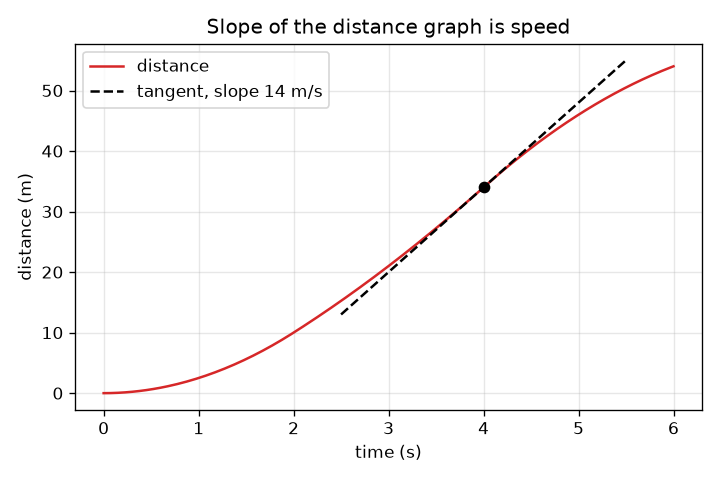
\includegraphics[width=0.85\linewidth]{figures/s01_distance_slope.png}\\\small Distance against time: the tangent at 4 s has slope 14 m/s, the speed.\end{center}

\subsection*{E. Worked example}
A car starts at rest and has speeds 10, 14 and 6 m/s at t = 2, 4 and 6 s, with straight lines between. Find the distance at each of those times, then the speed at t = 3 s and the slope of the distance graph there.
\begin{enumerate}[nosep]
\item Slice 1 (0 to 2 s): trapezoid with sides 0 and 10 m/s and width 2 s: (0 + 10)/2 * 2 = 10 m.
\item Slice 2 (2 to 4 s): (10 + 14)/2 * 2 = 24 m, so the distance at 4 s is 10 + 24 = 34 m.
\item Slice 3 (4 to 6 s): (14 + 6)/2 * 2 = 20 m, so the distance at 6 s is 54 m.
\item Speed at t = 3 s: half way between 10 and 14 m/s is 12 m/s.
\item Slope of the distance graph at 3 s: the distance changes by about 12 m for each second there, so the slope is 12 m/s, the same number. Unit check: m / s = m/s.
\end{enumerate}
\textbf{Answer.} Distances 10 m, 34 m and 54 m at 2, 4 and 6 s; speed 12 m/s at 3 s, equal to the slope of the distance graph there.

\subsection*{F. Questions}
\begin{enumerate}[nosep]
\item \textbf{Conceptual.} A friend says 'the speed graph is flat, so the car is not moving'. Is that right? What does a flat distance graph mean?
\item \textbf{Numerical.} A car has speeds 0, 12, 12 and 6 m/s at t = 0, 2, 4 and 6 s, with straight lines between. Find the total distance in 6 s and the average speed. Check the units.
\item \textbf{Graph and simulation interpretation.} In the distance graph of the car from the worked example (speeds 10, 14, 6 m/s), where is the curve steepest and what is its slope there? What is the slope at the end, t = 6 s?
\item \textbf{Design and optimisation challenge.} Design: choose the speeds at 2, 4 and 6 s (each at most 20 m/s, the limit of this exercise) so that the car covers at least 90 m in 6 s. Find a choice that works and one that fails, and say what you would trade off.
\end{enumerate}

\section{Session 2: Derivative and integral as limits}

\subsection*{A. Real-world problem}
A car's position is x(t) = 3 t\textasciicircum{}2 + 2 t metres, with t in seconds. What are its velocity and acceleration at 2 s, and are the units of every term sensible? Then a harder question: when a driver brakes, how far does the car go before it stops, and how fast can it be going if it must stop within 40 m?

\subsection*{B. Concept and theory}
The slope between two moments t and t + h is the secant slope (x(t + h) - x(t)) / h. As h gets smaller the secant slope settles on one number: the derivative x'(t), the slope of the tangent line. This 'settling' is called a limit. For x = 3 t\textasciicircum{}2 + 2 t at t = 2 the secant slope is 14 + 3 h, which tends to 14 m/s as h tends to 0. Rules: the derivative of c t\textasciicircum{}n is c n t\textasciicircum{}(n-1); of sin t is cos t; of e\textasciicircum{}t is e\textasciicircum{}t. Velocity is the derivative of position and acceleration is the derivative of velocity. For the integral, cut [a, b] into n slices of width dt = (b - a)/n and add up (height) * dt for each slice; as n grows the sum settles on the integral. The fundamental theorem says the integral of v from a to b equals x(b) - x(a) when v = x', so differentiating and integrating undo each other. Units: each term of x = 3 t\textasciicircum{}2 + 2 t must be in metres, so the 3 is in m/s\textasciicircum{}2 and the 2 in m/s. Braking: a steady slowdown a means the speed falls linearly from v0 to 0 in T = v0 / a, and the distance is the area of the triangle v0 T / 2 = v0\textasciicircum{}2 / (2 a). This is a simplified model: real braking depends on tyres, road and load and is not personal driving advice.

\begin{itemize}[nosep]
\item x(t): position of the car (m)
\item v(t) = x'(t): velocity (m/s)
\item a = v'(t): acceleration (m/s\textasciicircum{}2)
\item h: gap between the two moments of a secant (s)
\item n, dt: number and width of rectangles (no unit, s)
\item v0: speed when braking starts (m/s)
\item t\_r: driver reaction time before braking starts (s)
\end{itemize}

\begin{equation*}
x'(t)=\lim_{h\to 0}\frac{x(t+h)-x(t)}{h}
\end{equation*}

\begin{equation*}
\frac{d}{dt}\left(c\,t^n\right)=c\,n\,t^{n-1},\qquad \frac{d}{dt}\sin t=\cos t,\qquad \frac{d}{dt}e^t=e^t
\end{equation*}

\begin{equation*}
\int_a^b v(t)\,dt\approx\sum_{k=0}^{n-1}v(t_k)\,\Delta t,\qquad \Delta t=\frac{b-a}{n}
\end{equation*}

\begin{equation*}
\int_a^b x'(t)\,dt=x(b)-x(a)
\end{equation*}

\begin{equation*}
d_{\mathrm{stop}}=v_0\,t_r+\frac{v_0^2}{2a}
\end{equation*}

\begin{center}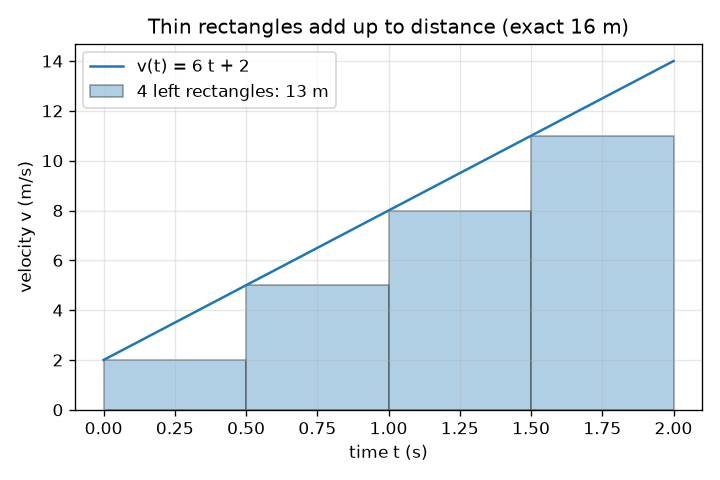
\includegraphics[width=0.85\linewidth]{figures/s02_riemann_rectangles.png}\\\small Four left rectangles under v = 6 t + 2: 13 m against the exact 16 m.\end{center}

\subsection*{E. Worked example}
For x(t) = 3 t\textasciicircum{}2 + 2 t (metres), find the velocity and acceleration at t = 2 s with units, check the derivative with secant slopes, and check the fundamental theorem on [0, 2] with rectangles.
\begin{enumerate}[nosep]
\item Position: x(2) = 3 * 4 + 2 * 2 = 12 + 4 = 16 m.
\item Velocity by the rule: v(t) = 6 t + 2, so v(2) = 14 m/s. Units: 6 is m/s\textasciicircum{}2 and times t (s) gives m/s; 2 is m/s.
\item Acceleration: a = v' = 6 m/s\textasciicircum{}2, constant.
\item Secant check at t = 2: slope = (x(2 + h) - x(2)) / h = 14 + 3 h, so h = 1 gives 17, h = 0.1 gives 14.3, h = 0.001 gives 14.003: tending to 14 m/s.
\item Fundamental theorem: the integral of v from 0 to 2 equals x(2) - x(0) = 16 m. Four left rectangles of width 0.5 s: heights v(0), v(0.5), v(1), v(1.5) = 2, 5, 8, 11 m/s, sum 26 * 0.5 = 13 m (below 16, as the curve rises); four midpoint rectangles give 16 m exactly because v is a straight line.
\end{enumerate}
\textbf{Answer.} x(2) = 16 m, v(2) = 14 m/s, a = 6 m/s\textasciicircum{}2; the secant slopes tend to 14 m/s and the rectangle sums tend to 16 m.

\subsection*{F. Questions}
\begin{enumerate}[nosep]
\item \textbf{Conceptual.} Why does the secant slope never equal the tangent slope exactly for h \textgreater{} 0, and why is it still useful to compute it?
\item \textbf{Numerical.} For x(t) = 5 t\textasciicircum{}2 + 4 t (metres), find x, the velocity and the acceleration at t = 3 s, with units, and check that the units of the two coefficients make sense.
\item \textbf{Graph and simulation interpretation.} In the position view with A = 3, B = 2, t = 2, the secant slope with gap h = 2 s is shown. What value do you read, and what happens when you reduce h to 0.1?
\item \textbf{Design and optimisation challenge.} Design: a driver has a reaction time of 0.75 s and the car brakes at a steady 6 m/s\textasciicircum{}2. What is the stopping distance from 25 m/s (90 km/h)? What is the largest speed that stops within 40 m? State two things this simple model leaves out.
\end{enumerate}

\section{Session 3: Numerical slopes and areas, and their errors}

\subsection*{A. Real-world problem}
A data logger gives numbers, not formulas. To get the acceleration or the distance from a speed record you must differentiate and integrate numerically, and every method makes an error. If you halve the step, how much better do you get? Can the step be too small? And when does a method fail entirely? We answer by testing four methods on functions whose exact answers we know.

\subsection*{B. Concept and theory}
Forward difference (f(x + h) - f(x)) / h has error roughly proportional to h (order 1). Central difference (f(x + h) - f(x - h)) / (2 h) has error roughly proportional to h\textasciicircum{}2 (order 2). Trapezoid rule joins neighbouring sample points by straight lines: error proportional to h\textasciicircum{}2 (order 2). Simpson's rule joins triples of points by parabolas: error proportional to h\textasciicircum{}4 (order 4), with an even number of slices. If error = C h\textasciicircum{}p then log(error) = log C + p log h, so on a log-log plot the points fall on a straight line of slope p: that is how we measure the order. For derivatives there is a second error: the computer stores numbers with about 16 digits, so f(x + h) - f(x) loses digits when h is tiny and the round-off error grows like 1e-16 / h. The total error falls and then rises; the best step sits at the bottom of the V. Methods assume the function is smooth; a corner or a narrow spike breaks the assumptions. Everything here is a simplified model with known exact answers, not a validated library.

\begin{itemize}[nosep]
\item h: step size (same unit as x)
\item n: number of slices, h = (b - a) / n (no unit)
\item p: order of a method: error \textasciitilde{} h\textasciicircum{}p (no unit)
\item tol: tolerance asked of the adaptive rule (same unit as the integral)
\item f(x): function being differentiated or integrated (any)
\end{itemize}

\begin{equation*}
f'(x)\approx\frac{f(x+h)-f(x)}{h}\ \ (\text{error}\sim h),\qquad f'(x)\approx\frac{f(x+h)-f(x-h)}{2h}\ \ (\text{error}\sim h^2)
\end{equation*}

\begin{equation*}
\int_a^b f\,dx\approx h\left[\tfrac12 f_0+f_1+\dots+f_{n-1}+\tfrac12 f_n\right]\ \ (\text{error}\sim h^2)
\end{equation*}

\begin{equation*}
\int_a^b f\,dx\approx\frac h3\left[f_0+4f_1+2f_2+4f_3+\dots+4f_{n-1}+f_n\right]\ \ (\text{error}\sim h^4)
\end{equation*}

\begin{equation*}
\log E\approx\log C+p\,\log h\quad\text{(slope }p\text{ on a log-log plot)}
\end{equation*}

\begin{center}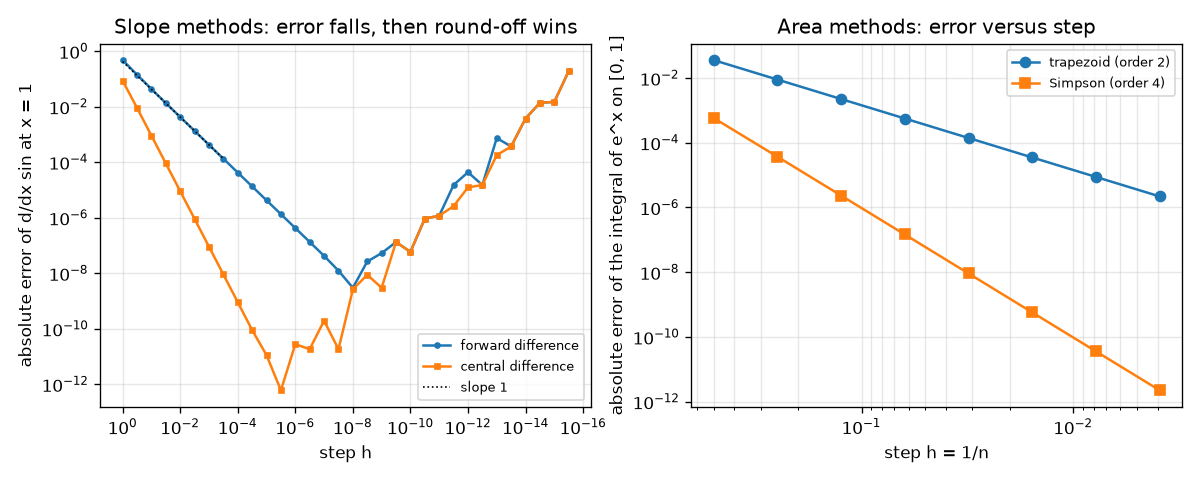
\includegraphics[width=0.85\linewidth]{figures/s03_error_vs_step.png}\\\small Left: slope errors fall with slopes 1 and 2 and then rise (round-off). Right: area errors fall with slopes 2 and 4.\end{center}

\subsection*{E. Worked example}
Find the forward and central difference of sin x at x = 1 with h = 0.1 and compare with the exact cos 1. Then find the trapezoid and Simpson areas of e\textasciicircum{}x on [0, 1] with n = 4 and compare with e - 1.
\begin{enumerate}[nosep]
\item Exact: cos 1 = 0.540302. Values: sin 1 = 0.841471, sin 1.1 = 0.891207, sin 0.9 = 0.783327.
\item Forward: (0.891207 - 0.841471) / 0.1 = 0.49736, error -0.0429. Central: (0.891207 - 0.783327) / 0.2 = 0.53940, error -0.0009. The central answer is about 48 times closer.
\item Areas: h = 0.25, values e\textasciicircum{}x = 1, 1.284025, 1.648721, 2.117000, 2.718282. Trapezoid: 0.25 * (0.5 + 1.284025 + 1.648721 + 2.117000 + 1.359141) = 1.727222, error +0.00894.
\item Simpson: (0.25 / 3) * (1 + 4 * 1.284025 + 2 * 1.648721 + 4 * 2.117000 + 2.718282) = 1.718319, error +0.000037. Exact e - 1 = 1.718282. Simpson is about 240 times closer with the same 5 points.
\item Pattern: with h = 0.01 the forward error is -0.0042 and the central error is -0.000009, in line with orders 1 and 2.
\end{enumerate}
\textbf{Answer.} Forward 0.49736 (error -0.0429) and central 0.53940 (error -0.0009); trapezoid 1.72722 (error 0.0089) and Simpson 1.71832 (error 0.000037).

\subsection*{F. Questions}
\begin{enumerate}[nosep]
\item \textbf{Conceptual.} Why can making the step h smaller make a numerical derivative worse?
\item \textbf{Numerical.} The trapezoid rule for e\textasciicircum{}x on [0, 1] with n = 16 has an error of 5.6e-4. Predict the error with n = 32, and for Simpson's rule if its error at n = 16 is 1.5e-7.
\item \textbf{Graph and simulation interpretation.} On a log-log plot of error against h, a method's points lie on a line which falls 4 decades while h falls 1 decade. What is its order? Which of our four methods is it?
\item \textbf{Design and optimisation challenge.} Design: you must integrate a function with one very narrow spike (width 0.005) on [0, 1] to 1e-8. Compare a uniform Simpson rule with an adaptive one, and say what could go wrong with the adaptive rule.
\end{enumerate}

\section{Real-world mini-project}
\textbf{Reconstruct the distance travelled from a noisy speedometer log.} A car's speedometer was logged 10 times per second for 60 s with \texttt{t, v = speedometer\_log()} from Session 3 (fixed seed 4, the default; the figures below are for that seed and are asserted by the Session 3 checkpoint). The log has random noise of 0.8 m/s and the speedometer reads 2 percent too high. The only outside fact is that a pair of roadside markers shows the car covered 822 m in the 60 s. Use \texttt{integrate\_log} to reconstruct the distance, remove the calibration error with the marker fact, and then estimate the car's acceleration by smoothing the speed before differentiating (a moving average of 21 samples is a good start).

\section{The path ahead}
\begin{enumerate}[nosep]
\item \textbf{Session 4: Romberg integration.} A Romberg table that builds higher-order rules from the trapezoid rule.
\item \textbf{Session 5: Gaussian quadrature.} A Gauss-Legendre integrator with a handful of nodes.
\item \textbf{Session 6: Derivatives without subtraction.} A derivative routine that avoids the round-off limit of Session 3.
\item \textbf{Session 7: Derivatives of noisy data.} A smoothing differentiator for the speedometer log of the mini-project.
\item \textbf{Session 8: Solve the braking ODE.} A solver for a braking car with drag, v' = -c v\textasciicircum{}2, and the distance it travels.
\end{enumerate}

\section{Answers and hints}

\subsection*{Session 1}
\begin{enumerate}[nosep]
\item \textbf{Conceptual.} Hint: Read the height of the speed graph, not its steepness, and remember slope = speed. Solution: No. A flat speed graph at 10 m/s means a constant speed of 10 m/s: the car is moving steadily, its distance graph is a straight sloped line (slope 10 m/s). A flat distance graph means the distance is not changing, so the speed is zero and the car is stopped. 'Flat' means different things on the two graphs: the speed graph shows the speed itself, the distance graph shows it only through its slope.
\item \textbf{Numerical.} Hint: Add three trapezoids; average speed is total distance divided by total time. Solution: Slice 1: (0 + 12)/2 * 2 = 12 m. Slice 2: (12 + 12)/2 * 2 = 24 m. Slice 3: (12 + 6)/2 * 2 = 18 m. Total = 54 m. Average speed = 54 m / 6 s = 9 m/s. Sanity check: the speed is always between 0 and 12 m/s, so 9 m/s is a believable average. Units: m/s * s = m.
\item \textbf{Graph and simulation interpretation.} Hint: The slope of the distance graph at a time equals the speed at that time. Solution: The curve is steepest at t = 4 s where the speed peaks at 14 m/s, so the slope is 14 m/s. At t = 6 s the speed is 6 m/s, so the slope has dropped to 6 m/s: the curve is still rising but much more gently. The distance never goes down because the speed is never negative.
\item \textbf{Design and optimisation challenge.} Hint: The total distance is 2 v1 + 2 v2 + v3 (three trapezoids). Try the largest speeds first. Solution: Total = 2 v1 + 2 v2 + v3. With 20, 20, 20: 40 + 40 + 20 = 100 m, which works. With 20, 20, 10: 90 m, just enough. With 15, 15, 15: 30 + 30 + 15 = 75 m, which fails. The first two speeds count double because they belong to two slices each, so being fast early matters most; the trade-off is that finishing at 20 m/s leaves less margin for stopping. Assumption: straight-line speed changes, no reversing.
\end{enumerate}

\subsection*{Session 2}
\begin{enumerate}[nosep]
\item \textbf{Conceptual.} Hint: Where does the secant line touch the curve, and what does a limit do? Solution: The secant line touches the curve at two points, so it measures the average slope over the gap h; the tangent line touches at one point. For x = 3 t\textasciicircum{}2 + 2 t at t = 2 the secant slope is 14 + 3 h, which is never 14 for h \textgreater{} 0. But it gets as close as we like by making h small, and that limit is the derivative. Computing secants is how computers estimate derivatives when no formula is known (Session 3).
\item \textbf{Numerical.} Hint: Use d/dt of c t\textasciicircum{}n = c n t\textasciicircum{}(n-1) twice. Solution: x(3) = 5 * 9 + 4 * 3 = 45 + 12 = 57 m. v(t) = 10 t + 4, so v(3) = 34 m/s. a = 10 m/s\textasciicircum{}2. Units: x is in m, so 5 is m/s\textasciicircum{}2 (m/s\textasciicircum{}2 * s\textasciicircum{}2 = m) and 4 is m/s (m/s * s = m). v = 10 t + 4 then has 10 in m/s\textasciicircum{}2 and 4 in m/s: m/s\textasciicircum{}2 * s = m/s. All terms are consistent.
\item \textbf{Graph and simulation interpretation.} Hint: The secant slope equals v + A h. Solution: With v = 14 m/s and A = 3 m/s\textasciicircum{}2 the secant slope is 14 + 3 * 2 = 20 m/s; with h = 0.1 it is 14.3 m/s. The secant line rotates towards the red tangent line as h shrinks. The secant is steeper than the tangent because the curve bends upwards (positive acceleration).
\item \textbf{Design and optimisation challenge.} Hint: Use d = v0 t\_r + v0\textasciicircum{}2 / (2 a). For the second part solve v t\_r + v\textasciicircum{}2 / (2 a) = 40 for v. Solution: From 25 m/s: reaction distance 25 * 0.75 = 18.75 m and braking distance 625 / 12 = 52.08 m, total about 70.8 m, far more than 40 m. For 40 m: v\textasciicircum{}2 / 12 + 0.75 v - 40 = 0, i.e. v\textasciicircum{}2 + 9 v - 480 = 0, so v = (-9 + sqrt(81 + 1920)) / 2 = 17.87 m/s, about 64 km/h. Check: 17.87 * 0.75 + 17.87\textasciicircum{}2 / 12 = 13.4 + 26.6 = 40 m. The model leaves out that real deceleration depends on tyres, road surface, slope and load, and that reaction times vary; it is a classroom model, not driving advice. The braking part grows as v\textasciicircum{}2, so doubling the speed quadruples it.
\end{enumerate}

\subsection*{Session 3}
\begin{enumerate}[nosep]
\item \textbf{Conceptual.} Hint: Think about f(x + h) - f(x) when the two numbers agree in their first 12 digits. Solution: When h is tiny, f(x + h) and f(x) are almost equal, and subtracting them cancels the leading digits, leaving only the few digits that are uncertain because the computer keeps about 16. Dividing by the tiny h then magnifies that round-off error by 1 / h. The method (truncation) error falls with h but the round-off error rises, so the total error has a minimum. In our test the forward difference is best near h = 1e-8 (error 3e-9) and the central near h = 3e-6 (error 6e-13); at h = 1e-15 both give an error of about 0.19.
\item \textbf{Numerical.} Hint: Doubling n halves h; error scales as h\textasciicircum{}p, so it is divided by 2\textasciicircum{}p. Solution: Trapezoid is order 2, so the error falls by a factor 2\textasciicircum{}2 = 4: about 1.4e-4. Simpson is order 4, so the error falls by 2\textasciicircum{}4 = 16: about 9e-9. Sanity check: Simpson at n = 16 is already about 4000 times more accurate than the trapezoid at the same n (5.6e-4 against 1.5e-7).
\item \textbf{Graph and simulation interpretation.} Hint: Slope = change in log error / change in log h. Solution: The slope is 4 (error falls by a factor 10\textasciicircum{}4 when h falls by 10), so the order is 4: Simpson's rule. Forward difference has slope 1, central difference and the trapezoid rule have slope 2.
\item \textbf{Design and optimisation challenge.} Hint: The adaptive rule splits slices only where its two estimates disagree. What if the first few samples all miss the spike? Solution: For the peak at 0.35 with width 0.005 the exact area is 0.0088623. Uniform Simpson reaches 1e-8 only with n = 512 slices (513 evaluations). Adaptive Simpson starting from 16 panels reaches the same accuracy with 424 evaluations, putting small slices at the spike. The risk: if the starting samples all miss the spike, the two estimates agree (both near 0) and the rule stops early with the wrong answer; that is why we start from 16 panels. The saving is moderate here and larger for narrower features. A 10-slice trapezoid reports 0.000000, wrong by 100 percent.
\end{enumerate}

\section{How to join}
Read \texttt{CONTRIBUTING.md} in the repository, then pick an issue labelled \texttt{good first issue}. Repository: \url{https://github.com/KrunalPanchal1995/opencalculus}

\end{document}
